
%(BEGIN_QUESTION)
% Copyright 2015, Tony R. Kuphaldt, released under the Creative Commons Attribution License (v 1.0)
% This means you may do almost anything with this work of mine, so long as you give me proper credit

Three-phase electric motors are often equipped with a set of electrical terminals for configuring different voltage ranges and/or base speeds.  Different configurations consist of different patterns of ``jumper'' wires connecting these terminals together.  For example, here is an illustration of a three-phase electric motor with nine stud-and-nut terminals for connecting a set of six wire windings (coils) in two different configurations: one for low voltage (240 volts AC) and one for high voltage (480 volts AC):

$$\includegraphics[width=15.5cm]{i03248x01.eps}$$

The following schematics show how the six windings interconnect for each voltage configuration, and how the three AC power conductors (A, B, and C) connect to supply AC power to these windings:

$$\includegraphics[width=15.5cm]{i03248x02.eps}$$

Sketch the proper power conductor and jumper connections for low-voltage operation and for high-voltage operation:

$$\includegraphics[width=15.5cm]{i03248x03.eps}$$

\vfil 

\underbar{file i03248}
\eject
%(END_QUESTION)





%(BEGIN_ANSWER)

This is a graded question -- no answers or hints given!
 
%(END_ANSWER)





%(BEGIN_NOTES)

This is just an exercise in connecting the dots!  A helpful problem-solving technique to apply to such problems is {\it tracing all connections made} in the schematic diagram after making those connections in the pictorial diagram.  This helps you keep track of which connections have been made, and which connections still need to be made.

$$\includegraphics[width=15.5cm]{i03248x04.eps}$$

%INDEX% Pictorial circuit review (3-phase motor connections)

%(END_NOTES)


